\section{Deep Learning Workloads}
Memory performance is an important factor that affects overall DNN performance, even in domain-specific architectures. 
For instance, TPU \mycite{jouppi2017tpu} shows that the array active cycle is 78.2\% with 86.0 TOPS/sec in CNN. 
The weight stall cycle is 0\% as CNNs reuse it in many domain-specific architectures. 
However, TPU performance is limited when executing MLP and RNN as they require high memory bandwidth. 
In MLP and LSTM, the weight stall cycle is 53.9\% and 58.1\% that fetches from memory. 
They try increasing memory bandwidth as four times, and the MLP and LSTM performance increase three times. 
Also, they found that higher memory bandwidth reduces on-chip memory pressure. 
We take CNNs, which is widely used DNNs, as an example. Most layers in CNNs consist of convolution (CONV) layer and fully connected (FC) layer.
Figure~\ref{fig:ch2:alg} (a) shows the base algorithm of FC layers, whose computation is general matrix-vector multiplication. 
The structure of data and weight are usually vector and matrix. Sequential as you see in the code, and it means DRAM access also shows sequential patterns. On the other hand, as shown in Figure~\ref{fig:ch2:alg} (b), traditional CNN compute 3D data and 4D weight matrix multiplication.

\begin{figure*}[ht]
    \centering
    \begin{minipage}[t][]{0.46\linewidth}
        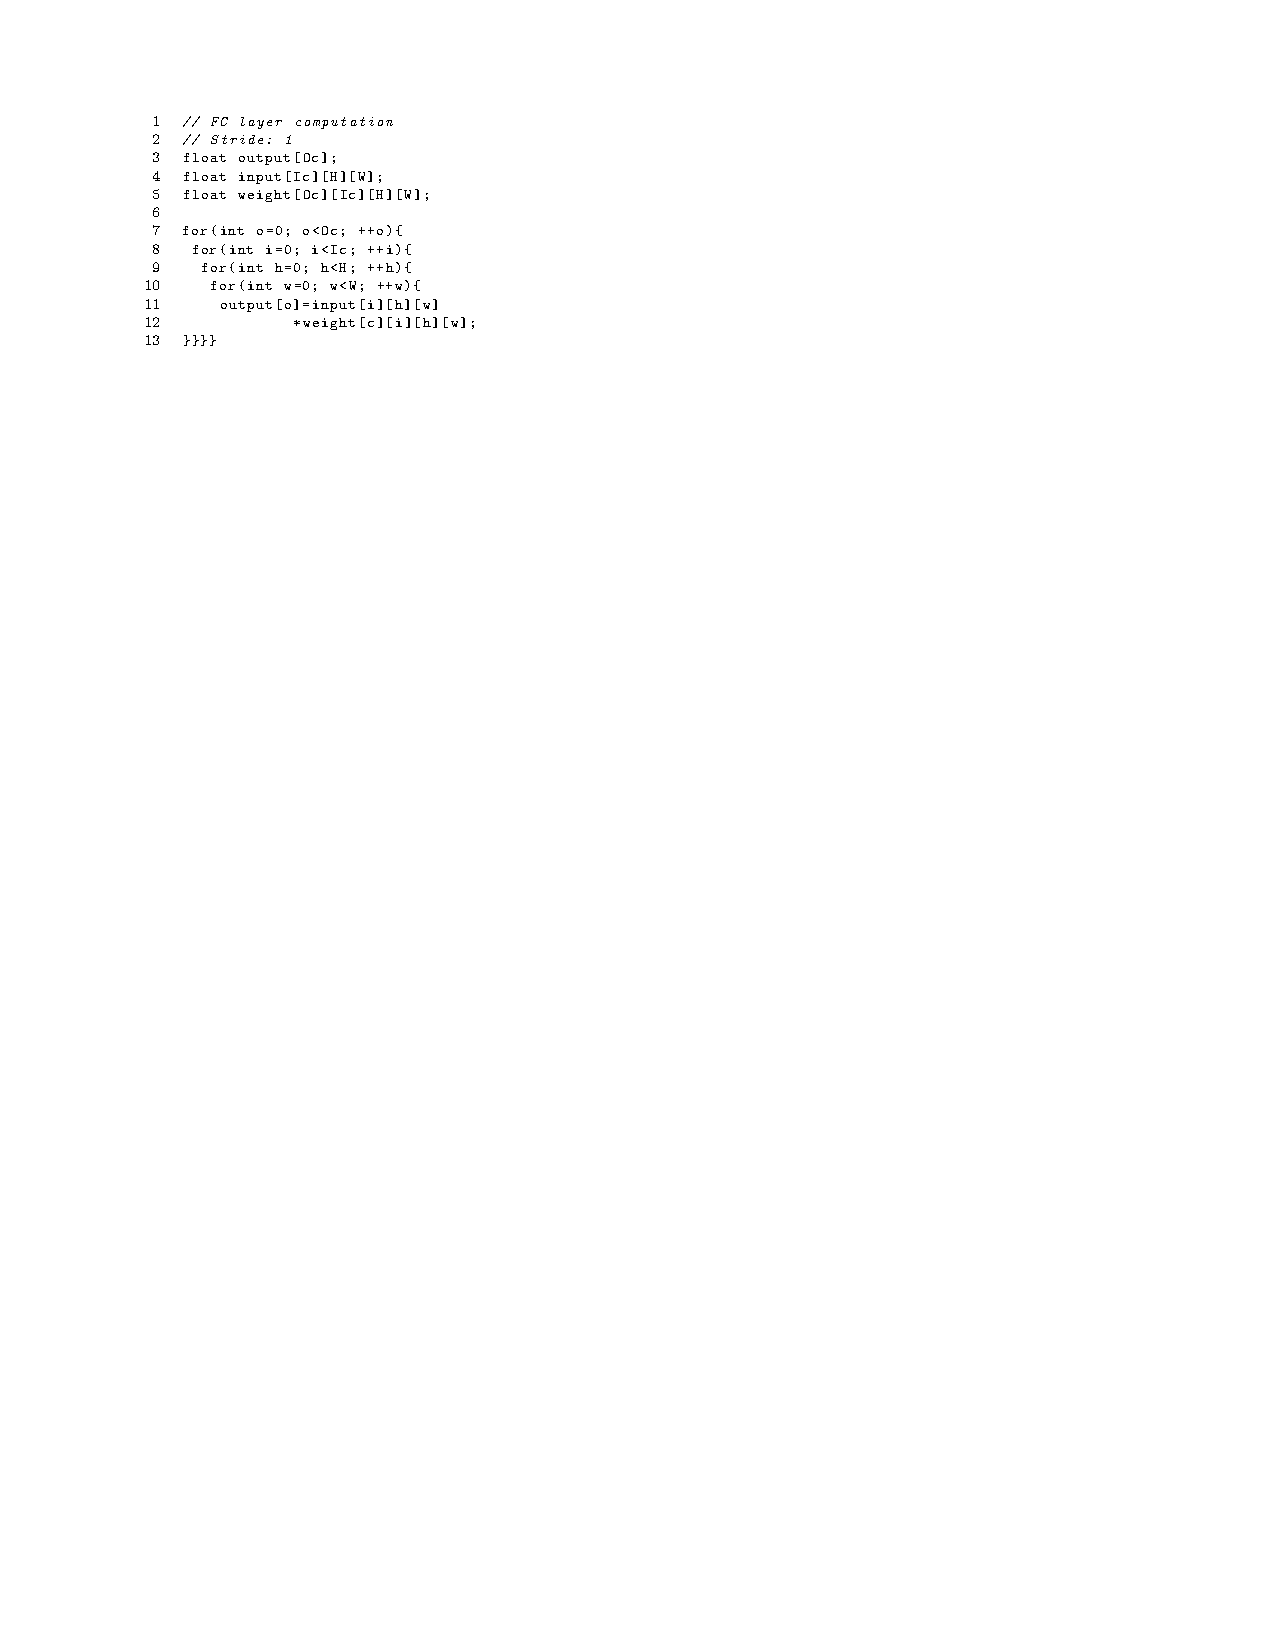
\includegraphics[]{figure/fc.pdf}
        \subcaption{FC layer computation}
    \end{minipage}
    \begin{minipage}[t][]{0.46\linewidth}
        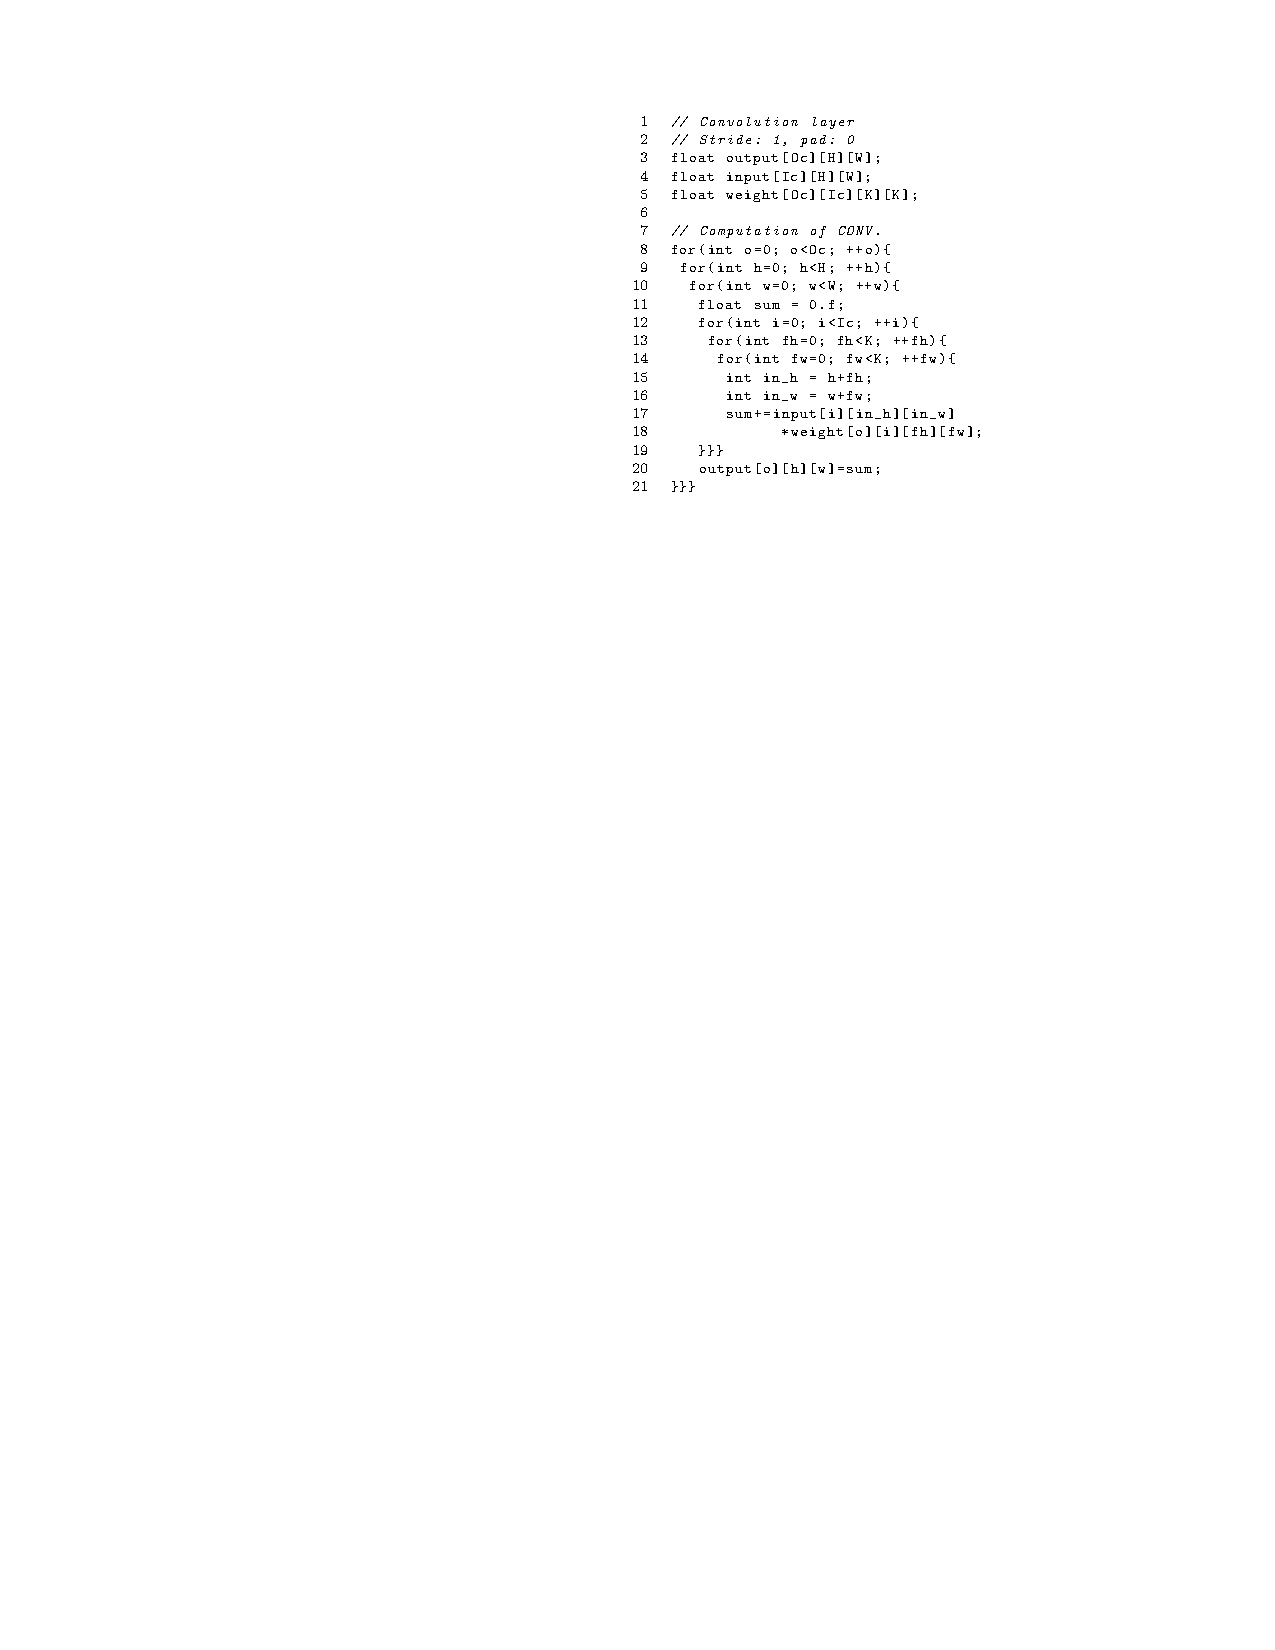
\includegraphics[]{figure/conv.pdf}
        \subcaption{CONV layer computation}
    \end{minipage}
    \caption{FC and CONV layer algorithms}
    \label{fig:ch2:alg}
\end{figure*}

It takes $O_{c}\times O_{h}\times O_{w}$ output multiplying $I_{c}\times I_{h}\times I_{w}$ 
data with $O_{c}\times I_{c}\times K_{h}\times K_{w}$ weight.
The convolution filter slides to each input features and accumulates to make one pixel of output feature.
In this computation, one convolution filter may meet an input pixel twice or more.
As this character, CNNs have two issue that decreases the GPU performance.
% 1. Out-Kernel: Duplication data and # of kernel.
First, there is a lot of duplicated data usage when computing convolution kernel parallel.
Weight is used for all input data and shared as thread index, but input data gets different thread and block index even though the value is same.
Also, GPUs should call lots of kernels computing each convolution as all matrix multiplication is independent.
These kernels are called at GPU core randomly and the memory access pattern is hard to predict what data to gather in the cache.
Besides, the GPU kernel size is bound to the convolution kernel size.
Most CNNs use convolution kernels with the size from $11\times 11$~\mycite{alex2012alexnet} to $1\times 1$~\mycite{he2016resnet} to get accurate features using the data.
This is significantly small compared to the maximum number of thread, usually 512 or 1024, in the kernel on GPU, and it causes the limitation of parallelism executing overall CNNs.
There is another issue when using small convolution kernels.
When it uses general $3\times 3$ convolution kernels, boundary check needs to compute the convolution kernel.
The condition flow in GPU is processed one-by-one execution and it decreases the GPU performance at least twice.
As memory access range is high in CNNs, it shows inefficient memory bandwidth.

\begin{figure*}[t]
    \centering
    \begin{minipage}[t][]{\linewidth}
        \centering
        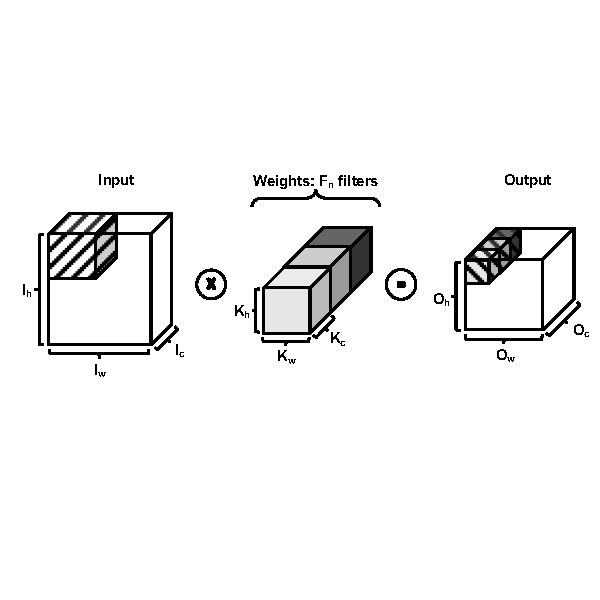
\includegraphics[width=0.9\linewidth]{figure/conv_lower1.pdf}
        \subcaption{Traditional convolution process}
    \end{minipage}
    \begin{minipage}[t][]{\linewidth}
        \centering
        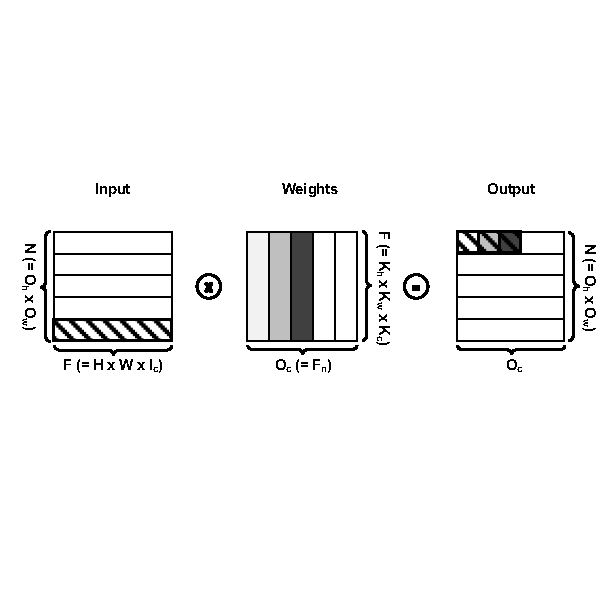
\includegraphics[width=0.9\linewidth]{figure/conv_lower2.pdf}
        \subcaption{Convolution lowering and computation}
    \end{minipage}
    \caption{Convolution structure and computation methodology}
    \label{fig:mot:conv}
\end{figure*}

To optimize memory bandwidth software transformations like convolutional lowering are performed to access memory sequentially.
cuDNN~\mycite{sharan2014cudnn} uses \texttt{im2col} function to convolutional lowering as depicted in Figure~\ref{fig:mot:conv} (b).
\texttt{$I_{c}\times I_{h}\times I_{w}$} input data is changed as \texttt{$I_{c}\times K_{h}\times K_{w}\times I_{h}\times I_{w}$} column.
After transforming, the convolution kernel executes general matrix multiplication (\texttt{GEMM}) with column and weight.
Though convolution lowering requires the amount of memory area due to saving the transformed matrix, it helps to serialize the GPU kernel and increase memory bandwidth as it does not check the boundary of the kernel and fetches continuous data.

\section{DRAM Access Patterns on GPU}
Both CONV (\texttt{im2col + GEMM}) and FC layers demonstrate largely sequential memory access patterns, to maximize DRAM bandwidth and minimize overfetching.
Figure~\ref{fig:ch2:pattern} (a) describes the last FC layer DRAM access patterns.
It reads DRAM on the regular step, which is the same as the stride of each data and weight values.
The output data is written at DRAM, in general, to pass over it to the next layer.
In this example, however, the output number of the last FC layer is only 10 that is small to remain the cache.
Also, it reuses directly at \texttt{softmax} function, which makes probability vector to prediction.
Hence, it does not have to access additional DRAM access to write the output.
In contrast, Figure~\ref{fig:ch2:pattern} (b) is divided into two sides; one for convolution lowering, and the other for matrix multiplication.
There are many DRAM write access (\texttt{0x81520000}~$\sim$~\texttt{0x81820000}) because of saving the transformed matrix data in the memory, while few DRAM read access (\texttt{0x81480000}~$\sim$~\texttt{0x814a0000}) to get original input data.
It might be possible to transform the data layout of a tensor to maximize row buffer locality. 
Although this approach has an advantage for deployment on commodity hardware, 
it is very difficult to implement it as it requires the knowledge of DRAM address mapping. 
Today's GPUs allocate some of the column address bits to high-order bits 
(with optional XOR address hashing) to minimize DRAM bank conflicts. 
This implies that even a simple one-dimensional array is interleaved over multiple banks 
in a non-contiguous manner. Thus, it is very challenging to optimize the data layout purely in software.
Besides, even if the data layout of a single array is carefully optimized, 
there are many concurrent thread blocks accessing the array out of order. 
The state-of-the-art SM scheduler does not take into account DRAM row buffer locality, and its 
non-deterministic behaviors make DRAM locality optimization in software even more difficult.

\begin{figure}[t]
	\centering
	\begin{minipage}{\textwidth}
	    \centering
    	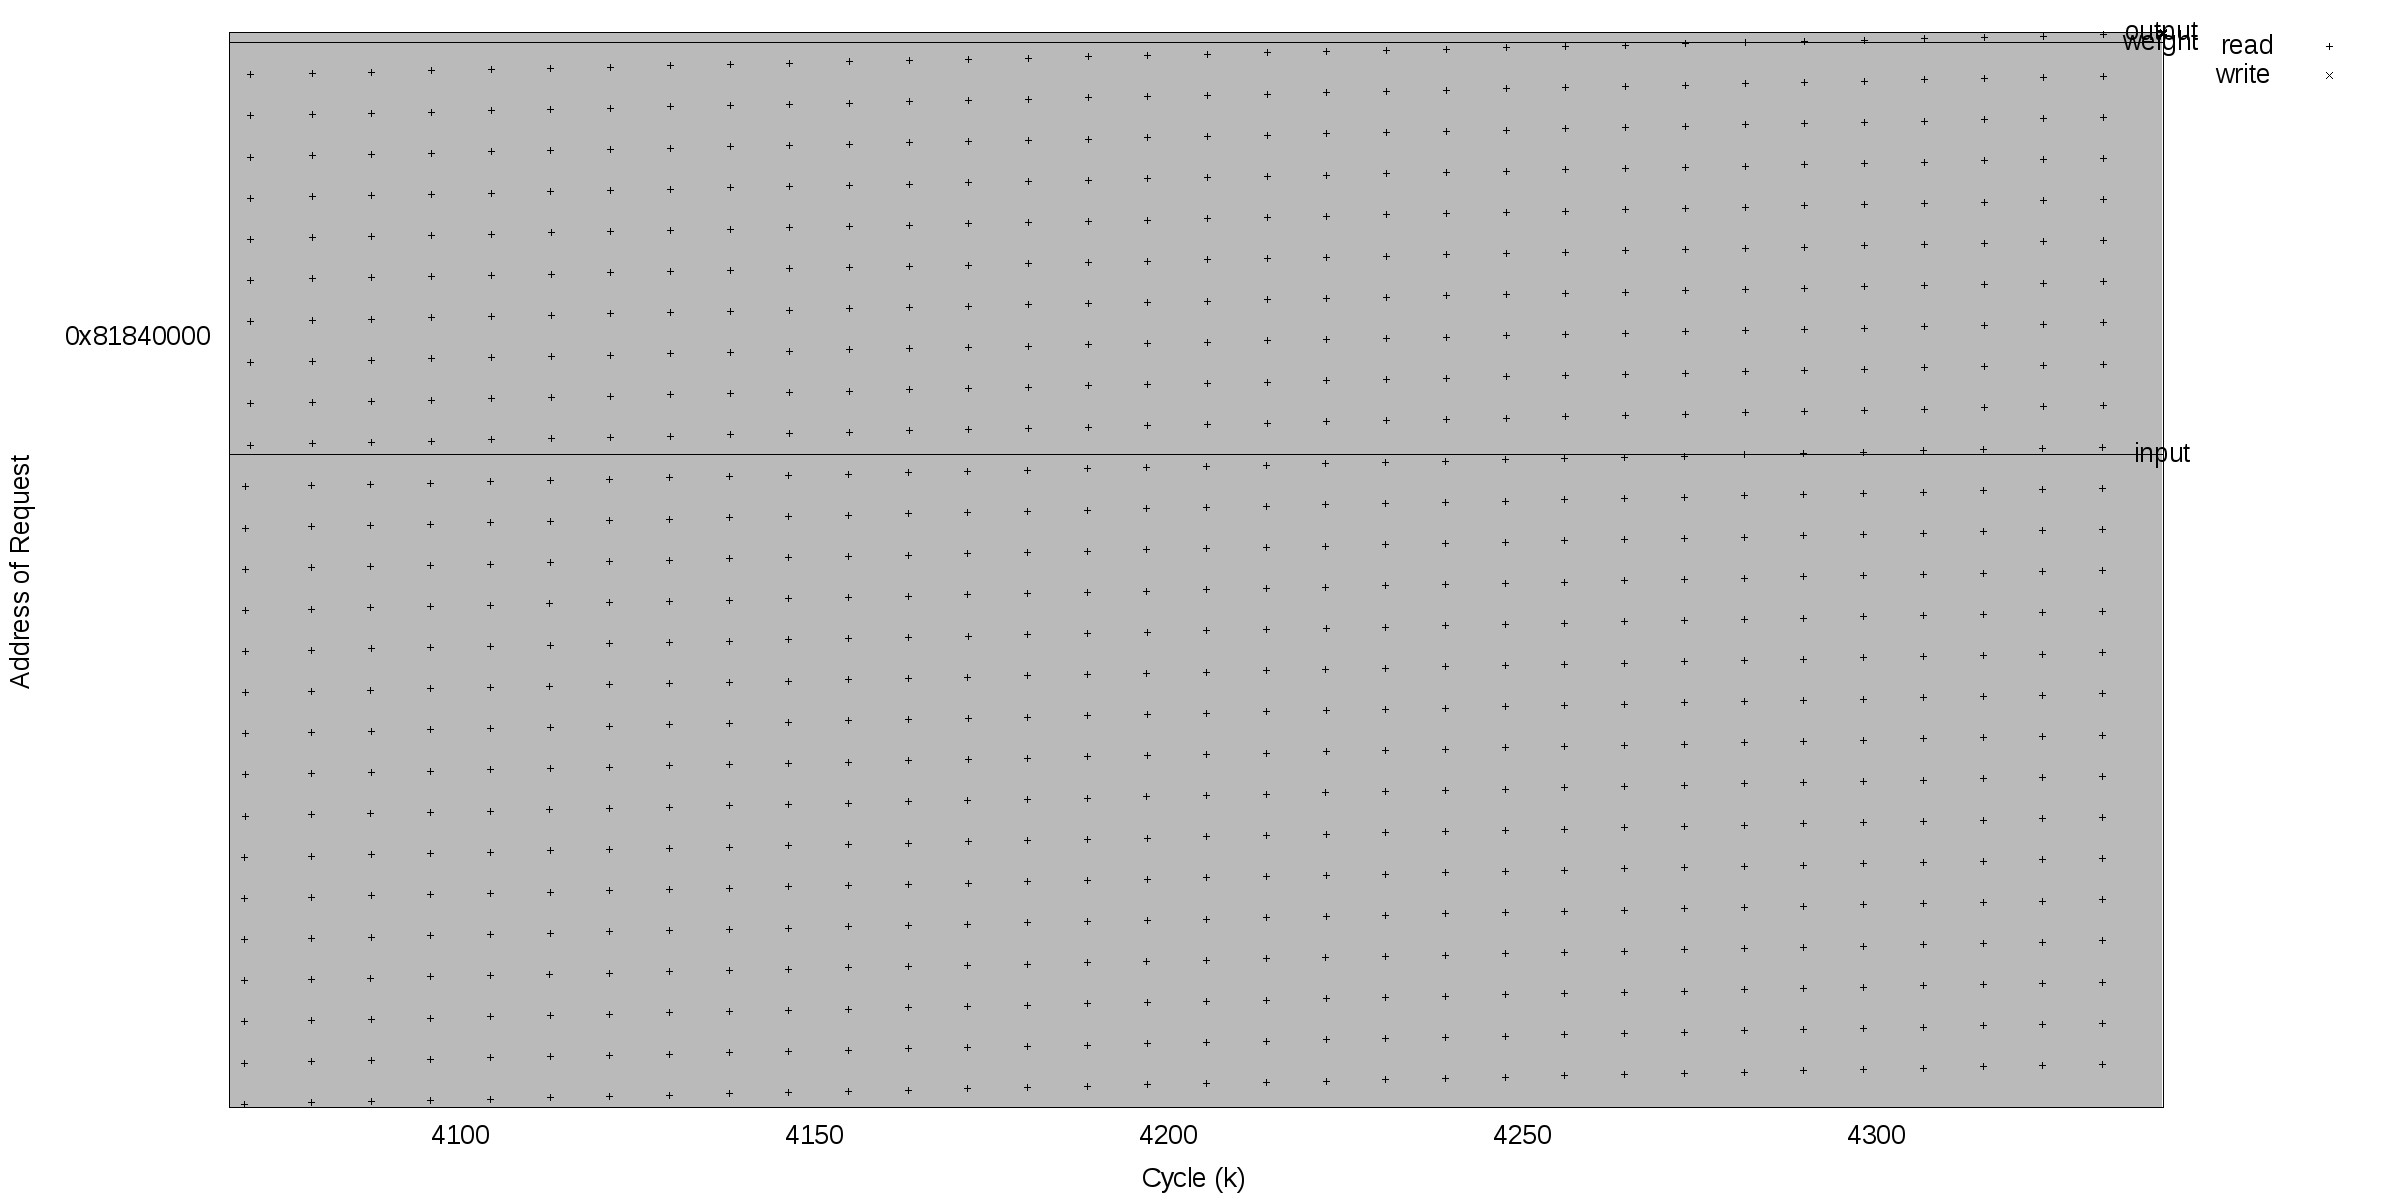
\includegraphics[width=0.80\textwidth]{figure/fcpat.png} 
    	\subcaption{FC layer}
    \end{minipage}	
	\begin{minipage}{\textwidth}
	    \centering
    	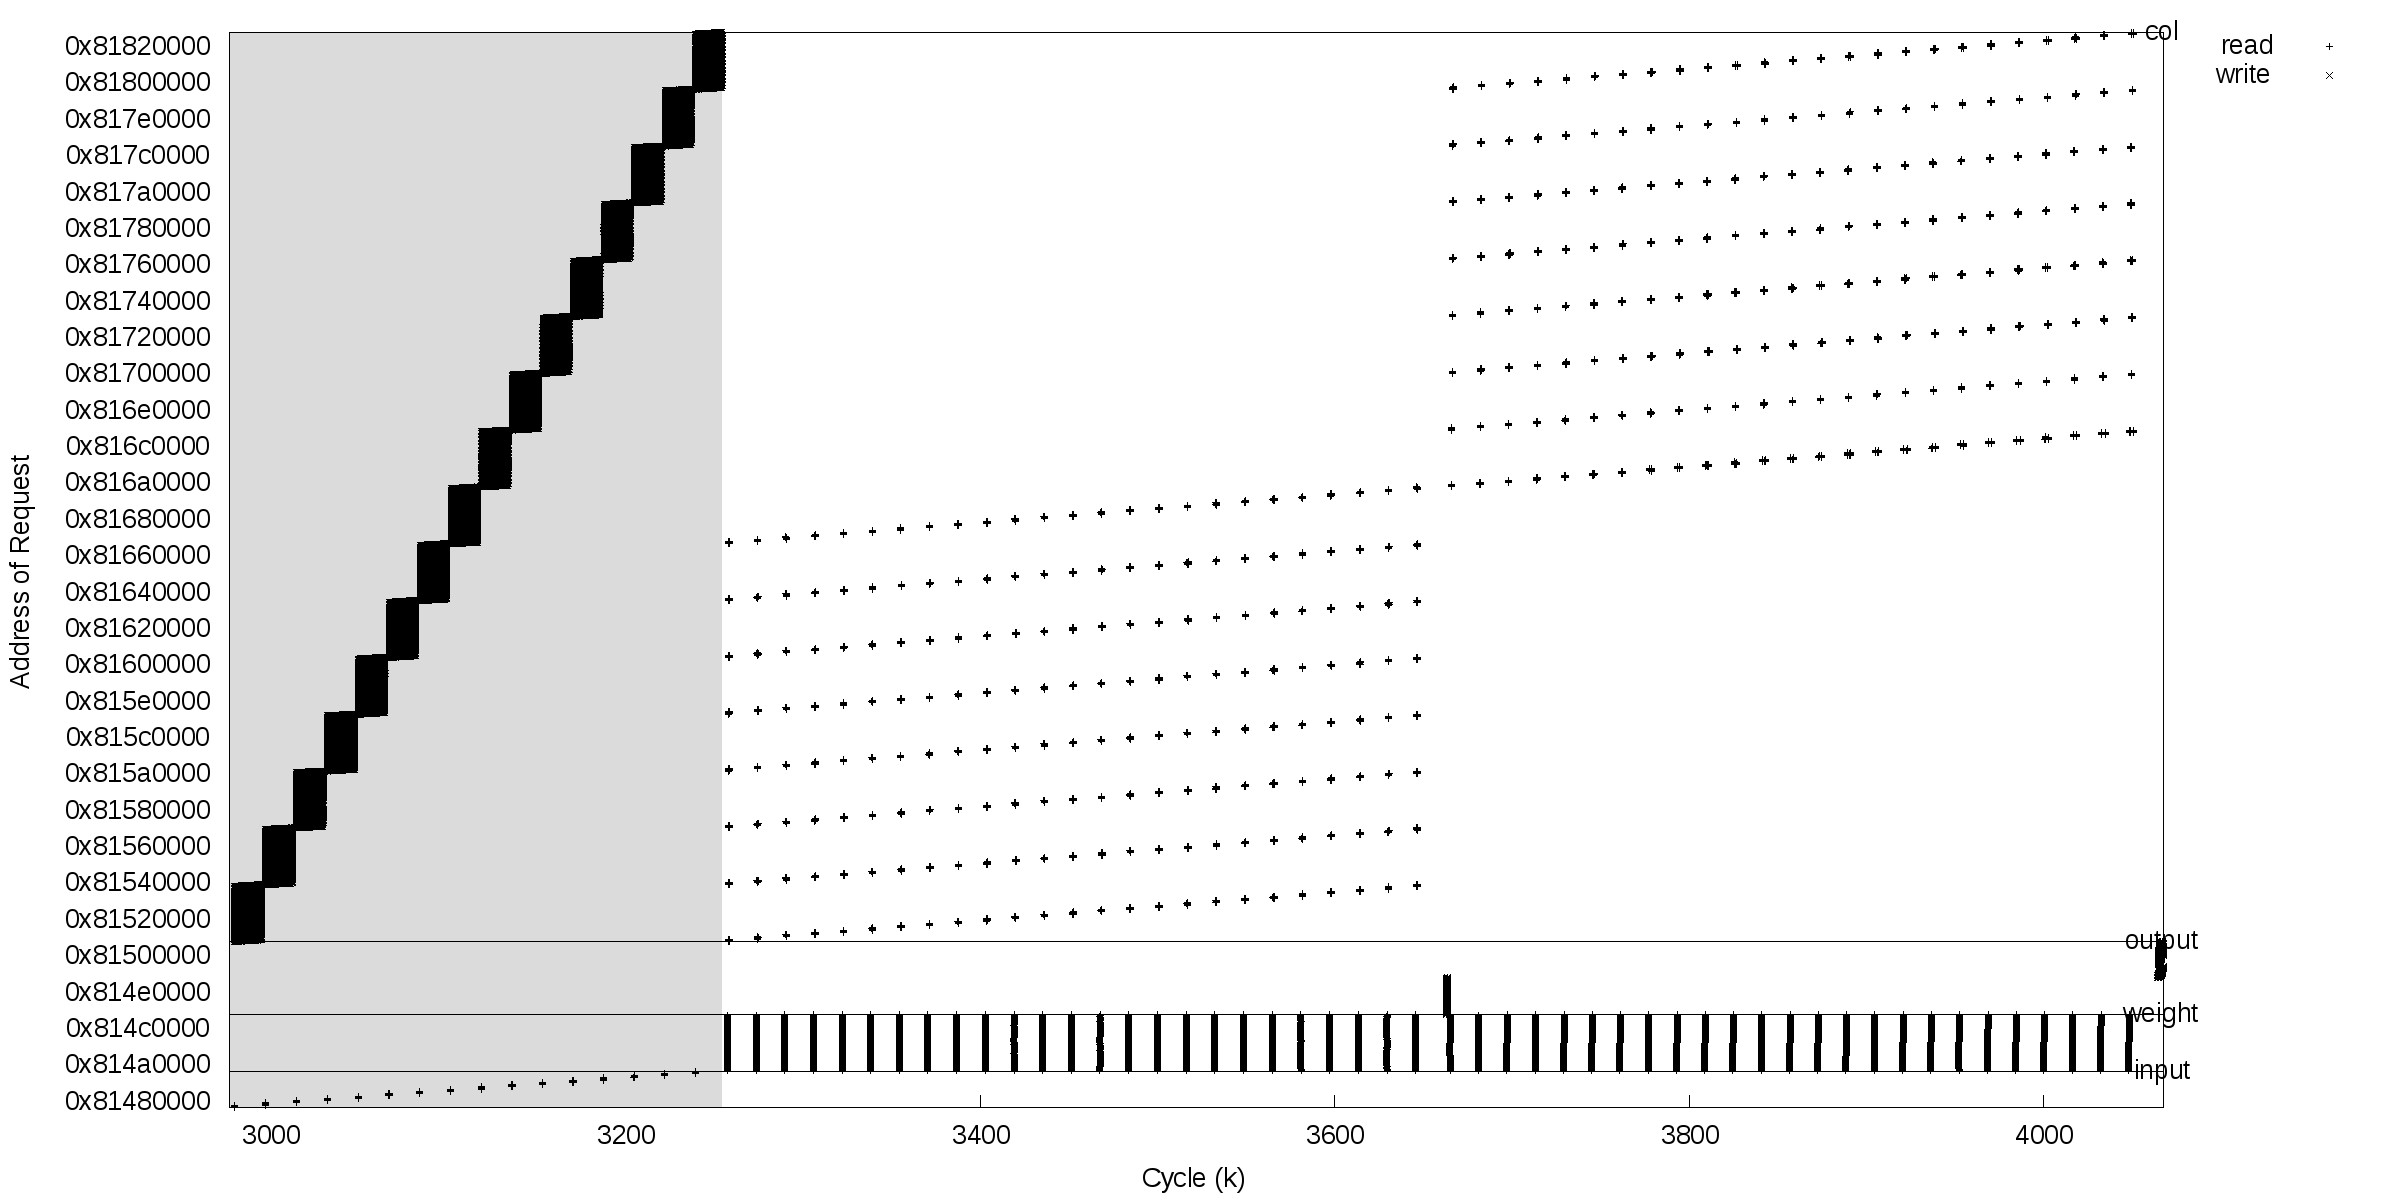
\includegraphics[width=0.80\textwidth]{figure/convpat.png}
    	\subcaption{CONV layer}
    \end{minipage}
	\caption{DRAM access patterns executing cuda-convnet on each layer}
	\label{fig:ch2:pattern}
\end{figure}

\section{Partial Row Activation}
Partial row activation scheme is a well-known technique to mitigate the overfetching problem.
Earlier works including Fujitsu Fast Cycle RAM (FCRAM)~\mycite{fcram}, fine-grained activation 
DRAM~\mycite{copper2010fineact} and~\mycite{udipi2010rethinking}.
These works can attain plenty of activation energy saving. 
However, that comes with a significant area overhead due to many peripherals 
(i.e., lower cell efficiency) which support fine-grained activation.
Fine-grained activation~\mycite{copper2010fineact} added a one-hot decoder and a single AND gate to the
wordline of each division in a row. The division of row is selected and activated when earning both 
row and column address. Using Posted-CAS command, DRAM controller sends row and column command 
back-to-back cycle. It reduced the DRAM power by up to 40\%. 

Selective bitline activation (SBA) and single subarray access (SSA)~\mycite{udipi2010rethinking}
fundamentally re-organized the layout of DRAM arrays and the mapping of data to these arrays so that an
entire cache line was fetched from a single subarray. Introducing new protocol existing JEDEC DRAM
interface called Posted-RAS, which hold the row address until the column address arrives to activate
the bitline selectively. It reduced dynamic and background energy about $5\times$.

More recent work addresses these problems but requires changes to the DRAM interface and protocols.
\mycite{yb17, Zhang14, halfpage, SALP12, subchannel17, connor2017finedram}
Many of these proposals make use of memory controller side information
when issue column commands (posted-CAS \mycite{postedcas}) or introduce new DRAM commands. 
\mycite{yb17}, for example, partial row activation mask is required
from the memory controller after row command issued to activate the dirty cache block.

Half-DRAM~\mycite{Zhang14} proposed a reconstructed DRAM architecture to address the row overfetching
problem. 
By splitting one mat into two parts, it enables half row activation which is almost no bandwidth
loss while achieving row activation power saving. As to the extending Half-DRAM which can perform
one-eighth row activation, it has a relatively large area overhead.

Fine-grained DRAM and subchannel~\mycite{connor2017finedram, subchannel17} proposed a new high-bandwidth
DRAM architecture to improves bandwidth by four times and energy efficiency by twice compared to existing
HBM2 reorganizing HBM2 channel structure into the narrow parallel channel to mitigate latency overhead 
due to the narrow path of the fine-grained activation structure. 
But these works require significant modification of microarchitecture of DRAM core that incurs 
the area overhead up to 10\%.

\section{Performance/Area Trade-off in Partial Activation}
 Many previous studies identify the row access energy as a major component of DRAM dynamic energy~\mycite{udipi2010rethinking, halfpage}. As a result, there are multiple proposals on partial row activation of DRAM. However, as we hinted earlier, most of these works require a substantial area overhead or changes to the DRAM protocol. This is because of a trade-off between cost (area) and performance. In a conventional DRAM architecture, a DRAM row is striped across multiple DRAM cell arrays, or \emph{mats}. Upon an {\tt ACTIVATE} command a whole row of each mat is latched. Then, when a {\tt READ} command arrives, each mat provides the same number of bits (i.e., 16 bits in HBM2 pseudo-channel mode) based on the provided column address from latches and outputs them to the bus. One potential way to enable partial activation is to segment every single row of each mat and activate only part of the selected row within a mat. However, this requires adding a large number of AND gates and local wordlines to incur huge area overhead~\mycite{udipi2010rethinking}. Another potential way is to re-arrange DRAM column data layout so that a single mat (or a few mats) contains the whole contents of a column in a row. This design can implement partial activation by letting only a single mat to be activated but it incurs a performance overhead as such design needs to output data through a narrow path between a single mat and the I/O, thus incurring serialization delay. An alternative to the previous approach is to increase the width of a path between a single mat and the bus to avoid performance penalty, which also results in a large area overhead.

\section{Latency-Tolerance of Deep Learning Workloads on GPU}
\begin{figure}[t]
	\centering
	    \centering
    	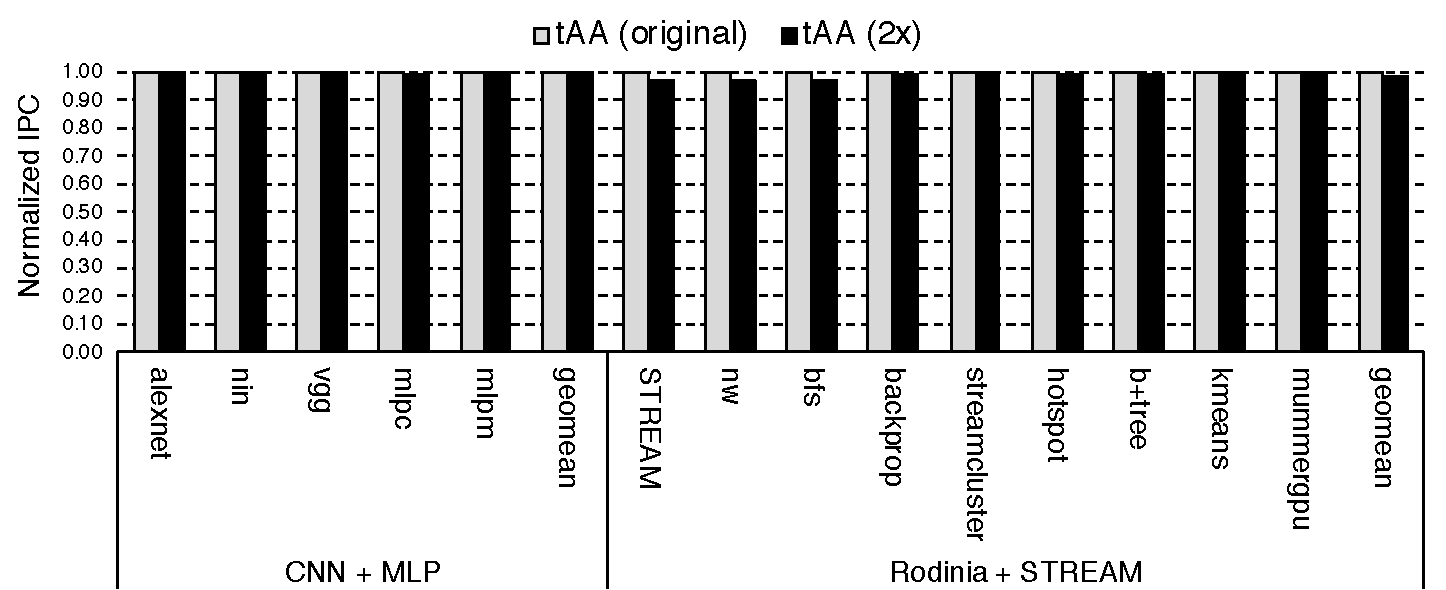
\includegraphics[width=0.90\textwidth]{figure/taa_long.pdf} 
	\caption{Performance degradation with longer column latency ({\tt tAA})}
	\label{fig:ch2:perfhit}
\end{figure}

 One important characteristic of the emerging GPU workloads is that they are tolerant to a long memory latency. Such workloads are often embarrassingly parallel and GPU exploits this characteristic by scheduling multiple warps (e.g., 64) to a single streaming multiprocessor (SM). When a warp in the SM cannot execute due to memory latency, another warp in the SM will be run instead. With this mechanism, the SM can effectively utilize its compute units and operate at a near-perfect efficiency despite the presence of long-latency memory operations. Figure~\ref{fig:ch2:perfhit} demonstrates the latency tolerance of two popular types of deep learning workloads, convolutional neural networks (CNNs) and multi-layer perceptrons (MLPs), by presenting the performance impact of increasing the {\tt tAA} timing parameter (i.e., internal read command to data output) by $2\times$. As shown in the figure, all five workloads show no performance degradation. The other conventional GPU workloads also show at most 4\% performance degradation. Note that this does not mean that the memory system is not important for GPU workloads. While they are less sensitive to memory latency, most GPU workloads, due to its high degree of parallelism, require large memory bandwidth. Based on this observation, we propose to trade DRAM latency for energy savings in this work.



%We need a more practical partial row activation scheme which has low area/power overhead without
%requiring changes to the existing DRAM interface.
%Unlike these previous works, our work avoids area overhead and significant interface change 
%while achieving substantial energy saving by exploiting the fact that most GPU workloads are not
%sensitive to memory latency.

